
% \section{Appendices}

\section*{Appendix A: Time plan}
\begin{figure}[ht]
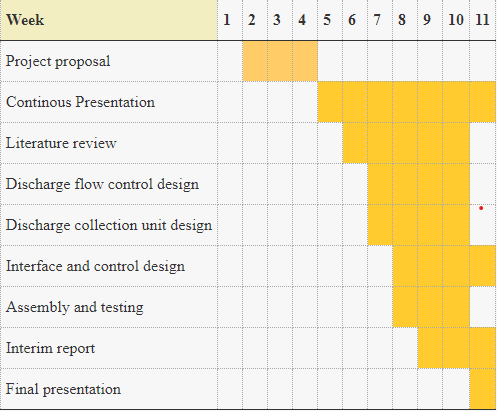
\includegraphics[width=\linewidth]{Figures/timeplan.png}
\centering
\end{figure}
\section*{Appendix B: Budget}
\begin{table}[ht]
  \begin{center}
    \leavevmode
     \begin{tabular}{|c | c | c | c | c |}\hline
      \textbf{Item No.} &  \textbf{Item} & \textbf{Quantity} & \textbf{Unit Cost} & \textbf{Cost} \\
     \hline
     001 & Flow Control valve & 1 & 1000 &  1000 \\
     \hline
     002 & Motor & 2 & 2500 &  5000 \\
     \hline
     003 & Limit Switch & 2 & 150 &  300 \\
     \hline
     004 & Temperature Probe & 1 & 300 &  300 \\
     \hline
     005 & Weight Sensors & 3 & 500 & 1500 \\
     \hline
     006 & DC Power Source & 1 & 1000 &  1000 \\
     \hline
     007 & Microcontroller &  1 & 6000 & 6000 \\
     \hline
     008 & Interface  & 1 & 2000  & 2000 \\
     \hline
     009 & Heat foil & 1 & 2000 & 2000 \\
     \hline
     \textbf{Total} & & & & 19100 \\
     \hline
    \end{tabular}
    \hangcaption{Budget}
    \label{table:1}
  \end{center}
\end{table}



    